\documentclass[compress,aspectratio=169]{beamer}

\mode<presentation>
{
  \usetheme{Singapore}
%  \setbeamertemplate{navigation symbols}{} % suppress nav bar
%  \setbeamercovered{transparent}
}

\usefonttheme{professionalfonts}
\usepackage{tikz}
\usepackage{amsmath}
\usepackage{mathpazo}
\usepackage[scaled]{helvet}
\usepackage{xcolor,colortbl}
\usepackage{siunitx}

\sisetup{
  number-math-rm=\mathnormal,
  per-mode=symbol
}

\title{Light Wave (Supplemental Slides)}
\subtitle{Advanced Placement Physics}
\author[TML]{Dr.\ Timothy Leung}
\institute{Olympiads School}
\date{Summer 2018}

\newcommand{\pic}[2]{\includegraphics[width=#1\textwidth]{#2}}
\newcommand{\half}{\ensuremath\frac{1}{2}}
\newcommand{\mb}[1]{\mathbf{#1}}
\newcommand{\eq}[2]{\vspace{#1}{\LARGE\begin{displaymath}#2\end{displaymath}}}

\begin{document}

\begin{frame}
  \maketitle
\end{frame}

\begin{frame}
  \frametitle{What These Slides Are About}
  These slides are condensed from the Grade 12 Physics slides for the unit on
  \emph{The Wave Nature of Light}. Some of the information are also
  presented in other classes.
\end{frame}

%\begin{frame}
%  \frametitle{In This Unit}
%  In this unit, we will be discussing some important properties of light:
%  \begin{itemize}
%  \item Light waves passing through a medium
%    \begin{itemize}
%    \item Reflection
%    \item Refraction
%    \item Dispersion
%    \end{itemize}
%  \item Light waves passing through an opening
%    \begin{itemize}
%    \item Diffraction
%    \item Interference
%    \item Optical resolution
%    \end{itemize}
%  \item The nature of light? (What kind of wave is light?)
%    \begin{itemize}
%    \item Maxwell's equations
%    \item Electromagnetic waves
%    \item Polarization of light
%    \item Speed of light
%    \end{itemize}
%  \end{itemize}
%  Some of the topics that we are discussing are reviews\ldots but with new
%  insights and more information.
%\end{frame}

\section{Huygens}
\begin{frame}
  \frametitle{Huygens' Principle}
  In the 1600's there were two competing theories of light\ldots
  \begin{itemize}
  \item Some, including Issac Newton, believed that  light is a particle
  \item Others, including Christiaan Huygen (Dutch) and Augustin-Jean Fresnel
    (French), believed that light is a wave
  \end{itemize}
  \vspace{.4in}

  Huygen's Princple: all waves are in fact an infinite series of circular
  wavelets
\end{frame}

\section{Reflection}
\begin{frame}
  \frametitle{Reflection of Light}
  \textbf{Law of Reflection}
  
  The incident ray, the reflected ray, and the normal to the surface of the
  mirror all lie in the same plane, and the angle of reflection is equal to
  the angle of incidence.  
  \begin{center}
    \pic{.7}{Types-of-reflection.jpg}
  \end{center}
\end{frame}

\begin{frame}
  \frametitle{Specular Reflection}
  \framesubtitle{Example: Lake Reflection}
  \begin{center}
    \pic{.55}{Lake-reflection.jpg}
  \end{center}
  This photo of Lake Matheson shows specular reflection in the water of the
  lake with reflected images of Aoraki/Mt Cook (left) and Mt Tasman (right).
  The very still lake water provides a perfectly smooth surface for this to
  occur.
\end{frame}

\section{Refraction}

\begin{frame}
  \frametitle{Refraction of Light Through a Medium}
  \begin{columns}
    \column{.4\textwidth}
    \begin{itemize}
    \item When a wave enters another medium, the wave speed changes
    \item When entering at an angle, the change of speed causes the wave to
      change direction (e.g.\ from air to water, air to glass, glass to air etc)
    \item The amount of bending depends on the
      \textbf{indices of refraction of the two media}
    \item Responsible for \textbf{image formation} by lenses and the eye
    \end{itemize}
    \column{.6\textwidth}
    \pic{1}{negative_refraction.jpg}
  \end{columns}
\end{frame}

\begin{frame}
  \frametitle{Refraction of Light Through a Medium}
    You have probably all seen this diagram of light entering from one medium
    to another.
    \begin{center}
      \pic{.3}{snells_interface.png}
    \end{center}
    Light could be going in either direction, from top to bottom ($n_1$ to
    $n_2$) or from bottom to top ($n_2$ to $n_1$)
\end{frame}

\begin{frame}
  \frametitle{Refraction Happens in Ocean Waves Too!}
  \begin{center}
    \pic{.5}{refraction-water-waves.png}
  \end{center}
  Refraction happens not only with light, we see the same behaviour in ocean
  waves, when the wave travel from deeper water (faster waves) to shallow
  depths.
\end{frame}

\begin{frame}
  \frametitle{Refraction and Huygens Principle}
  \begin{columns}
    \column{.5\textwidth}
    \pic{1}{huygen.png}
    \column{.47\textwidth}
    We can explain the refraction phenomenon using Huygens' Principle
  \end{columns}
\end{frame}

\begin{frame}
  \frametitle{Snell's Law}

  \textbf{Snell's law} relates the indices of refraction $n$ of the two media
  to the directions of propagation in terms of the angles to the normal. 

  \vspace{-.2in}
  {\Huge
    \begin{displaymath}
      \boxed{n_1\sin\theta_1=n_2\sin\theta_2}
    \end{displaymath}
  }
  
  \vspace{.1in}
  \begin{center}
    \begin{tabular}{l|c|c}
      \rowcolor{pink}
      \textbf{Variable} & \textbf{Symbol} & \textbf{SI Unit}\\ \hline
      Indices of refraction of the media & $n_1$, $n_2$ & (no units)\\
      Incident angle of light   & $\theta_1$ & (no units)\\
      Refraction angle of light & $\theta_2$ & (no units)\\
    \end{tabular}
  \end{center}
\end{frame}

\begin{frame}
  \frametitle{Index of Refraction}

  \textbf{Index of refraction} ($n$) is defined as the speed of light in vacuum
  ($c$) divided by the speed of light in the medium ($v$).

  \eq{-.2in}{
    \boxed{n=\frac{c}{v}=\frac{\lambda_\mathrm{vacuum}}{\lambda}}
  }

  When light enters a second medium, the \emph{frequency} remains
  unchanged (i.e.\ the colour doesn't change!) but since the speed changes,
  the \emph{wavelength} also changes:
    
  \eq{-.2in}{
    \boxed{\frac{n_1}{n_2}=\frac{\lambda_2}{\lambda_1}}
  }
\end{frame}

\begin{frame}
  \frametitle{Index of Refraction of Common Materials}
  \begin{center}
    \begin{tabular}{c|c||c|c}
      \rowcolor{pink}
      \textbf{Material} & \textbf{n} & \textbf{Material} & \textbf{n}\\ \hline
      Vacuum           & 1        & Ethanol     & 1.362 \\
      Air              & 1.000277 & Glycerine   & 1.473 \\
      Water at \SI{20}{\celsius} & 1.33 & Ice         & 1.31 \\
      Carbon disulfide & 1.63     & Polystyrene & 1.59 \\
      Methylene iodide & 1.74     & Crown glass & 1.50-1.62\\
      Diamond          & 2.417    & Flint glass & 1.57-1.75\\
    \end{tabular}
  \end{center}
  
  \vspace{.2in}
  The values given are \emph{approximate} and do not account for the small
  variation of index with light wavelength which is called
  \textbf{dispersion}. We'll get to that later!
\end{frame}

\begin{frame}
  \frametitle{Total Internal Reflection}
  \framesubtitle{From High Index to Low Index}
  Snell's law still holds, but something weird can happen:
  \begin{center}
    \pic{.8}{660px-RefractionReflextion.png}
  \end{center}
  Critical angle $\theta_c$ for water-air interface is \ang{48.6}. If
  incident angle is greater $\theta_1>\theta_c$, we have
  \textbf{total internal reflection}. TIR can only happen going from a higher
  index to a lower index, $n_1>n_2$.
\end{frame}

\section{Dispersion}

\begin{frame}
  \frametitle{Colour of Light and Wavelength}
  Human eyes perceive different frequencies of light as different colours.
  The visible spectrum of light:
  \begin{center}
    \pic{.45}{visiblespectrum.png}
  \end{center}
  \begin{itemize}
  \item The ``colour'' of the light depends on its frequency (\& wavelength
    when it's in a vacuum)
  \item \emph{White light} is light that contains waves in all frequencies.
  \end{itemize}
\end{frame}

\begin{frame}
  \frametitle{Dispersion of Light Through Refraction}
  \begin{columns}
    \column{.4\textwidth}
    \pic{1}{white-light-split.jpg}
    \column{.55\textwidth}
    \begin{itemize}
    \item When white light passes through a prism it is separated into
      different colours (spectrum) through refraction.
    \item This is because the index of refraction $n$ is slightly different for
      different wavelengths
    \item Otherwise, we will never see a rainbow
    \end{itemize}
  \end{columns}
\end{frame}

\begin{frame}
  \frametitle{Wavelength Dependency of Index of Refraction}
  \begin{center}
    \pic{.5}{Dispersion-curve.png}
  \end{center}
\end{frame}

\begin{frame}
  \frametitle{Chromatic Aberration}
  \framesubtitle{This is What Disperson Can Do!}
  When looking at an image through a low-quality binocular, magnifying glass, or
  telescope, we often see the edges of images blurred a bit. Sometimes we see
  a rainbow-coloured edge:
  \begin{center}
    \pic{.5}{choosing03-pic002.png}
  \end{center}
  Chromatic Aberration can occur even with high-quality camera lenses,
  particularly with wide-angle lenses where light from high angles have to bend
  towards the camera sensor/film, requiring high lens curvature.
\end{frame}

\begin{frame}
  \frametitle{Chromatic Aberration}
  \framesubtitle{This is What Disperson Can Do!}
  The reason that chromatic aberration happens is the same reason that prisms
  work: \textbf{dispersion of light}
  \begin{center}
    \pic{.5}{chromatic-aberration.jpg}
  \end{center}
  The focal lengths for different frequencies (colour) of light are different,
  thus blurring the image. So how do we fix it?
\end{frame}

\begin{frame}
  \frametitle{Chromatic Aberration: Camera Lens Design}
  By lining different lenses of different materials and geometries, we can
  correct for the chromatic aberration.
  \begin{center}
    \pic{.5}{Apochromatic-Lens.png}
  \end{center}
  \begin{itemize}
  \item Lens design is a closely guarded secret by camera companies
  \item Shape of the lens, material and coating are all factors
  \item A ``lens'' on a DSLR camera can have up to 30 lens ``elements''
  \end{itemize}
\end{frame}


\section{Interference}

\begin{frame}
  \frametitle{Thomas Young's Double-Slit Experiment}
  \framesubtitle{First definitive evidence that light is a wave}
  \begin{columns}
    \column{.45\textwidth}
    \pic{1}{double-slit1.png}
    \column{.52\textwidth}
    \begin{itemize}
    \item\textbf{Monochromatic light} light with a single colour (frequency);
      the light source can be a laser, LED , or gas lamp (most likely what Young
      used)
    \item\textbf{Slit:} an opening; also called an \textbf{aperture}
    \item The \textbf{screen} far away from the slits is also called the
      \textbf{projection}
    \end{itemize}
  \end{columns}

  \vspace{.15in}Double-slit experiment showed that light causes interference,
  just like any other wave
\end{frame}

\begin{frame}
  \frametitle{Thomas Young's Double-Slit Experiment}
  \begin{columns}
    \column{.3\textwidth}
    \pic{1.2}{path1.png}
    \column{.7\textwidth}
    \begin{itemize}
    \item At \textbf{A}, the path from slits $S_1$ and $S_2$ are the same,
      therefore \textbf{constructive interference} (bright fringe)
    \item At \textbf{B}, the path from $S_1$ and $S_2$ differ by half a
      wavelength, and therefore \textbf{destructive interference} (dark fringe)
    \item At \textbf{C}, the path from $S_1$ and $S_2$ differ by one
      wavelength, and therefore \textbf{constructive interference} (bright
      fringe) again
    \end{itemize}
  \end{columns}
\end{frame}

\begin{frame}
  \frametitle{Interference Pattern: Bright and Dark Fringes}
  \begin{center}
    \pic{.4}{fringes1.png}
  \end{center}
  The ``bright fringes'' are from constructive interference; the ``dark
  fringes'' are from destructive interference.
\end{frame}


\begin{frame}
  \frametitle{Double-Slit Interference}
  \begin{columns}
    \column{.5\textwidth}
    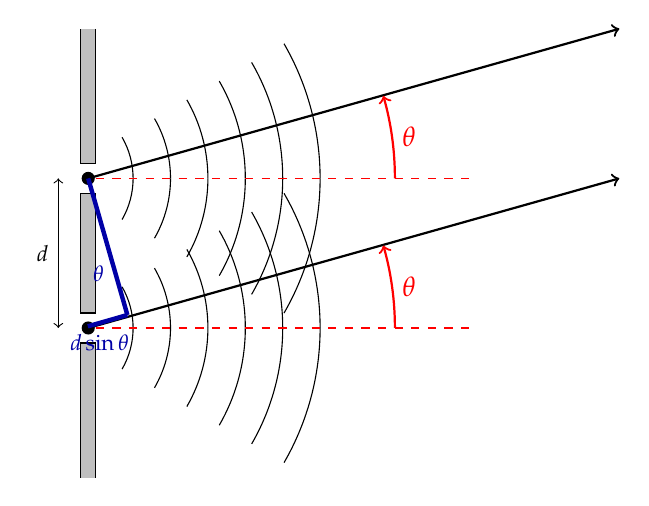
\begin{tikzpicture}[scale=.95]
      \draw[fill=gray!50](0,3)--(0,1.2)--(-.2,1.2)--(-.2,3);
      \draw[fill=gray!50](0,.8)--(0,-.8)--(-.2,-.8)--(-.2,.8)--cycle;
      \draw[fill=gray!50](0,-3)--(0,-1.2)--(-.2,-1.2)--(-.2,-3);
      \draw[<->](-.5,-1)--(-.5,1) node[midway,left]{\footnotesize $d$};
      %\draw[dashed](0,0)--(8,0);

      \draw[fill=black](-.1,1) circle(.08);
      \draw[fill=black](-.1,-1)circle(.08);
      \foreach \x in {.5,1,...,3} {
        \pgfmathsetmacro\xx{\x+.6};
        \draw(\x,1) arc(0:30:\xx); \draw(\x,1) arc(0:-30:\xx);
        \draw(\x,-1)arc(0:30:\xx); \draw(\x,-1)arc(0:-30:\xx);
      }
      \draw[thick,->](-.1,1)--(7,3);
      \draw[thick,->](-.1,-1)--(7,1);

      \draw[red,thick,->](4,1) arc(0:16:4) node[midway,right]{$\theta$};
      \draw[red,thick,->](4,-1)arc(0:16:4) node[midway,right]{$\theta$};
      \draw[red,dashed](0,1)--(5,1);
      \draw[red,dashed](0,-1)--(5,-1);

      \begin{scope}[rotate around={16:(-.1,1)}]
        \draw[blue!65!black,ultra thick](-.1,1)--(-.1,-.9)
        node[pos=.7,left]{\footnotesize $\theta$};
        \draw[blue!65!black,ultra thick](-.1,-.9)--(-.65,-.9)
        node[pos=.7,below]{\footnotesize $d\sin\theta$};
      \end{scope}
    \end{tikzpicture}
    \column{.47\textwidth}
    \begin{itemize}
    \item We have two slits at distance $d$ apart, emitting \emph{coherent}
      light
    \item Huygens' Principle: light passing through the slits become
      point sources
    \item Assume that the projection (screen) is far enough from the slits
      that we can treat the two beams of light from the slits as being parallel
    \item Using basic geometry, we can see that the path difference from the
      two slit to the projection is $d\sin\theta$
    \end{itemize}      
  \end{columns}
\end{frame}

\begin{frame}
  \frametitle{Double-Slit Interference}
  \framesubtitle{Constructive Interference}
  A bright fringe (constructive interference) occurs when the path difference
  ($d\sin\theta$) is an integer ($n$) multiple of wavelength ($\lambda$), i.e.
  
  \eq{-.2in}{
    \boxed{\pm n\lambda = d\sin\theta_n}
  }

  Conversely, a dark fringe (destructive interference) occurs when the path
  difference ($d\sin\theta$) is a half-number ($n+\frac{1}{2}$) multiple of
  wavelength ($\lambda$), i.e.
  
  \eq{-.2in}{
    \boxed{\pm\left(n+\frac{1}{2}\right)\lambda = d\sin\theta_n}
  }
  where $n=0,1,2,3\ldots$

\end{frame}

\begin{frame}
  \frametitle{Double-Slit Interference}
  \begin{center}
    \pic{.65}{path-difference.png}
  \end{center}
  %The path difference between slits that light has to travel to reach the screen
  %is given by $d\sin\theta$.
\end{frame}

\begin{frame}
  \frametitle{Approximation of The Wavelength of Light}
  We can estimate the wavelength of light based on the distances between bright
  fringes, by applying the \textbf{small-angle approximation} (make sure
  $\theta$ is in \emph{radians}):

  \eq{-.25in}{
    \theta\approx\tan\theta\approx\sin\theta
  }
  
  \vspace{-.15in}The distance from slits to the screen ($x$), and the distance
  of the $n$-th bright fringe from the centre ($y_n$) to $\theta_n$ can be
  approximated by:

  \eq{-.2in}{
    \tan\theta_n=\frac{y_n}{x}\approx\sin\theta_n
  }
  
  \vspace{-.1in}We can substitute our approximation into the constructive
  interference equation:

  \eq{-.2in}{
    n\lambda\approx\frac{y_nd}{x}
    \quad\longrightarrow\quad
    \boxed{\lambda\approx\frac{\Delta y d}{x}}
  }
\end{frame}

\begin{frame}
  \frametitle{Approximation of The Wavelength of Light}
  This equation applies equally to dark fringes (nodal lines) as well as bright
  fringes.
  
  \eq{-.2in}{
    \boxed{\lambda\approx\frac{\Delta y d}{x}}
  }
  \begin{center}
    \begin{tabular}{l|c|l}
      \rowcolor{pink}
      \textbf{Quantity} & \textbf{Symbol} & \textbf{SI Unit} \\ \hline
      Wavelength                     & $\lambda$  & \si{\metre} (metre) \\
      Distance between fringes       & $\Delta y$ & \si{\metre} (metre) \\
      Distance between slits         & $d$        & \si{\metre} (metre) \\
      Distance from slits to screen & $x$        & \si{\metre} (metre) \\
    \end{tabular}
  \end{center}

  Since the approximation is based on small angles, we generally apply this
  to $\Delta y$ close to the centre, where light from both slits are deflected
  by a small angle.
\end{frame}


\begin{frame}
  \frametitle{Important Notes}
  \begin{itemize}
  \item We have applied the double-slit problem specifically to light, but it
    can be applied to any wave (e.g.\ ocean waves) as well
  \item The ``slits'' don't actually need to be slits; any point source will do
  \item The projection/screen doesn't need to be a real screen either; it just
    has to be a line where wave intensity can be measured
  \end{itemize}
\end{frame}

\section{Diffraction}

\begin{frame}
  \frametitle{Diffraction of Waves}
  When a wave goes through an small opening, it \textbf{diffracts}. This happens
  with sound waves, ocean waves\ldots and light.
  \begin{center}
    \pic{.6}{alexandria.jpg}
  \end{center}
  (The photo is from the Port of Alexandria in Egypt. The shape of the entire
  harbour is created because of diffraction of ocean wave.)
\end{frame}

\begin{frame}
  \frametitle{Diffraction of Waves}
  \begin{center}
    \pic{.6}{diffraction1.jpg}
  \end{center}
  The smaller the opening (compared to the wavelength of the incoming wave)
  the greater the diffraction effects.
\end{frame}

\begin{frame}
  \frametitle{There are Two Types of Diffraction}
  \begin{itemize}
  \item\textbf{Fresnel diffraction}
    \begin{itemize}
    \item ``Near-field'' diffraction
    \item The distance between aperture and the projection is small
    \item The short distance to the projection causes the diffraction pattern
      observed to differ in size and shape
    \end{itemize}
  \item\textbf{Fraunhofer diffraction}
    \begin{itemize}
    \item ``Far-field diffraction''
    \item The distance between the aperture and the projection is large
    \item Will only focus on this form of diffraction in Physics 12 because
      the pattern is easier to understand
    \end{itemize}
  \end{itemize}
\end{frame}

\begin{frame}
  \frametitle{Fresnel Number}
  The Fresnel number tell us when to use Fresnel diffraction (difficult) and
  when to use Fraunhofer (easier):

  \vspace{-.3in}{\huge
    \begin{displaymath}
      F=\frac{W^2}{\lambda L}
    \end{displaymath}
  }
  \begin{center}
    \begin{tabular}{l|c|l}
      \rowcolor{pink}
      \textbf{Quantity} & \textbf{Symbol} & \textbf{SI Unit} \\ \hline
      Fresnel Number        & $F$         & (no units) \\
      Characteristic length of the aperture & $W$ & \si{\metre} (metres)\\
      Wavelength of light   & $\lambda$           & \si{\metre} (metres)\\
      Distance from aperture to projection & $L$  & \si{\metre} (metres)\\
    \end{tabular}
  \end{center}

  \begin{itemize}
  \item Fresnel diffraction if $F\gg 1$; Fraunhofer diffraction if $F\ll 1$
  \item In Physics 12, we will only deal with Fraunhofer diffraction
  \end{itemize}
\end{frame}

\begin{frame}
  \frametitle{Let's Work This Out Again!}
  \begin{columns}
    \column{.4\textwidth}
    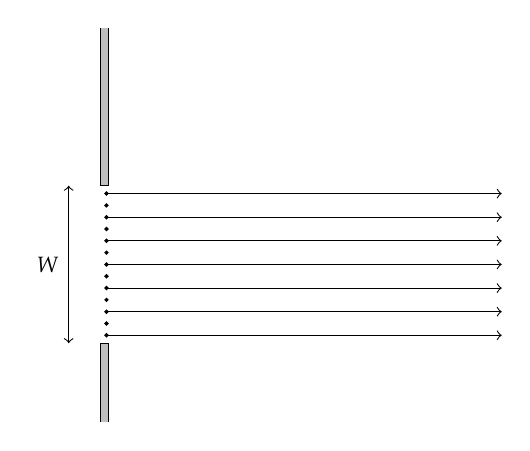
\begin{tikzpicture} %[scale=.95]
      \draw[fill=gray!50](0,3)--(0,1)--(-.1,1)--(-.1,3);
      \draw[fill=gray!50](0,-2)--(0,-1)--(-.1,-1)--(-.1,-2);
      \draw[<->](-.5,-1)--(-.5,1) node[midway,left]{\footnotesize $W$};
      \foreach \y in {1,...,13} {
        \pgfmathsetmacro\yy{1.05-.15*\y};
        \draw[fill=black](-.02,\yy) circle(.02);
      }
      \foreach \y in {1,3,...,13} {
        \pgfmathsetmacro\yy{1.05-.15*\y};
        \draw[->](-.02,\yy)--(5,\yy);
      }
    \end{tikzpicture}
    \column{.57\textwidth}
    \begin{itemize}
    \item Similar to the double-slit problem, we apply Huygens' Principle
      again
    \item Treat the slit as wide enough that there is an infinite series of
      point waves at the slit
    \item The light from the wavelet that travel perpendicular to the aperture
      will not interfere with one another
    \item i.e.\ a bright fringe at the middle called the
      \textbf{central maximum}.
    \end{itemize}
  \end{columns}
\end{frame}




\begin{frame}
  \frametitle{At Some Angle $\theta$}
  \begin{columns}
    \column{.4\textwidth}
    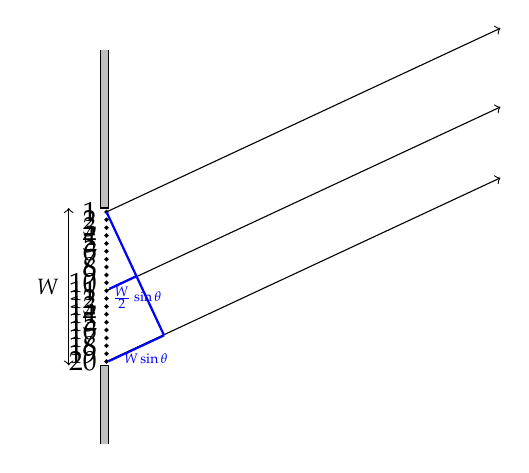
\begin{tikzpicture} %[scale=.95]
      \draw[fill=gray!50](0,3)--(0,1)--(-.1,1)--(-.1,3);
      \draw[fill=gray!50](0,-2)--(0,-1)--(-.1,-1)--(-.1,-2);
      \draw[<->](-.5,-1)--(-.5,1) node[midway,left]{\footnotesize $W$};
      \foreach \y in {1,...,20} {
        \pgfmathsetmacro\yy{1.05-.1*\y};
        \draw[fill=black](-.02,\yy) circle(.02) node[left]{\Tiny\y};
        }
      \foreach \y in {1,11,20} {
        \pgfmathsetmacro\yy{1.05-.1*\y};
        \draw[->,rotate around={25:(-.02,\yy)}](-.02,\yy)--(5.5,\yy);
      }
      \begin{scope}[rotate around={25:(-.02,.95)}]
        \draw[blue,thick](-.02,.95)--(-.02,-.78);
        \draw[blue,thick](-.02,-.78)--(-.8,-.78)
        node[pos=.9,right]{\tiny $W\sin\theta$};
        \draw[blue,thick](-.02,.05)--(-.4,.05)
        node[pos=0,below]{\tiny $\frac{W}{2}\sin\theta$};
      \end{scope}
    \end{tikzpicture}
    \column{.57\textwidth}
    \begin{itemize}
    \item Repeating the analyis as double-slit, we can find the path
      difference between the wavelet on the top (1) and bottom
      (20): $W\sin\theta$
    \item At some $\theta$, the path difference between 1 and 20 will be one
      wavelength ($\lambda$)
    \item In this case, the path difference between 1 and 11 is
      half of the wavelength (i.e.\ destructive interference) and they cancel
      each other
    \item Similarly, 2 cancels 12, 3 cancels 13\ldots, resulting in
      \textbf{complete desctructive interference}
    \end{itemize}
  \end{columns}
\end{frame}


\begin{frame}
  \frametitle{Dark Fringes: Destructive Interference}
  Dark fringes exists on the screen at regular, whole-numbered intervals
  ($m=1,2,3\ldots$):

  \eq{-.2in}{
    \boxed{\pm m\lambda=W\sin\theta_m}
  }
  
  \vspace{-.15in}Applying small-angle approximation equation, we end up with:

  \eq{-.2in}{
    \boxed{y_m=\frac{m\lambda L}{W}}
  }
  
  \fbox{
    \begin{minipage}{.96\textwidth}
      \textbf{Pro-tip:} This equation looks very similar to the double-slit
      equation for \emph{bright} fringes, so be \emph{very} careful when you
      use them!
    \end{minipage}
  }
\end{frame}


\begin{frame}
  \frametitle{At Some Other Angle $\theta$}
  \begin{columns}
    \column{.4\textwidth}
    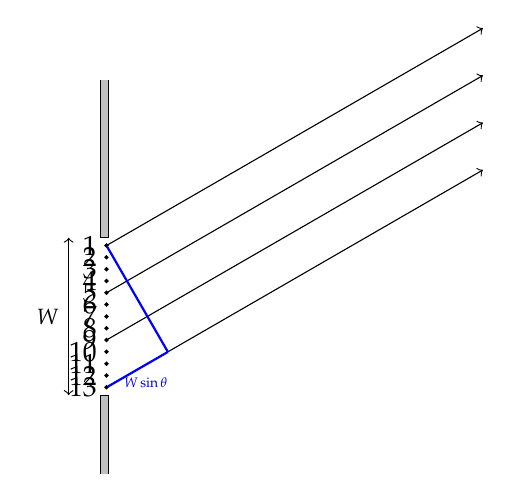
\begin{tikzpicture} %[scale=.95]
      \draw[fill=gray!50](0,3)--(0,1)--(-.1,1)--(-.1,3);
      \draw[fill=gray!50](0,-2)--(0,-1)--(-.1,-1)--(-.1,-2);
      \draw[<->](-.5,-1)--(-.5,1) node[midway,left]{\footnotesize $W$};
      \foreach \y in {1,...,13} {
        \pgfmathsetmacro\yy{1.05-.15*\y};
        \draw[fill=black](-.02,\yy) circle(.02) node[left]{\Tiny\y};
        }
      \foreach \y in {1,5,9,13} {
        \pgfmathsetmacro\yy{1.05-.15*\y};
        \draw[->,rotate around={30:(-.02,\yy)}](-.02,\yy)--(5.5,\yy);
      }
      \begin{scope}[rotate around={30:(-.02,.9)}]
        \draw[blue,thick](-.02,.88)--(-.02,-.66);
        \draw[blue,thick](-.02,-.66)--(-.9,-.66)
        node[pos=.9,right]{\tiny $W\sin\theta$};
      \end{scope}
    \end{tikzpicture}
    \column{.57\textwidth}
    \begin{itemize}
    \item Again, we follow what we did with the the previous case, and we
      find that at some angle $\theta$, the path difference between the top
      and bottom is $W\sin\theta=\frac{3}{2}\lambda$
    \item Beam from (1) and (5) differ by $\frac{\lambda}{2}$, so they
      have destructive interference; similarly 2 and 6, 3 and 7, 4 and 8,
      9 and 13 will all interfere destructively
    \item But some of the beams will not, so we have a bright fringe at the 
      projection
    \item This bright fringe is not as bright as the central one because
      of the destructive interference
    \end{itemize}
  \end{columns}
\end{frame}



\begin{frame}
  \frametitle{Bright Fringes: Constructive Interference}
  Bright fringes exist on the screen at regular, half-numbered intervals
  ($m=1,2,3\ldots$):

  \eq{-.2in}{
    \boxed{\pm\left(m+\half\right)\lambda=W\sin\theta_m}
  }
  
  \vspace{-.1in}Again, similar to the dark fringes, we apply our small-angle
  approximation equation:

  \eq{-.2in}{
    \boxed{y_m=\pm\left(m+\half\right)\frac{\lambda L}{W}}
  }
\end{frame}


\begin{frame}
  \frametitle{Single-Slit Diffraction, A Summary}
  \begin{itemize}
  \item Similar to the double-slit interference, single-slit diffraction
    projects a series of alternating bright fringes (``maxima'') and dark
    fringes (``minima'') in the far field
  \item The bright fringe in the middle (``central maximum'') is twice as wide
    and very bright
  \item Subsequent bright fringes on either side (``higher-order maxima'') are
    much dimmer because of the partial destructive interference
  \end{itemize}
  \begin{center}
    \pic{.65}{Single_Slit_Diffraction.png}
  \end{center}
\end{frame}

\section{Grating}
\begin{frame}
  \frametitle{Diffraction Grating: What if there are more than 2 slits?}
  \begin{columns}
    \column{.38\textwidth}
    \pic{1}{grating1.jpg}
    \column{.62\textwidth}
    \begin{itemize}
    \item We can apply the same analysis from double-slit to a diffraction
      grating
    \item Use equation for double-slit interference to locate bright fringes
      
      \vspace{-.2in}{\Large
        \begin{displaymath}
          n\lambda=d\sin\theta_n
        \end{displaymath}
      }
    \item Interference pattern is sharper
    \item Bright fringes are narrower
    \end{itemize}
  \end{columns}
\end{frame}

\section{Applications}

\begin{frame}
  \frametitle{Resolving Power}
  The ability of an optical instrument (e.g.\ the human eye, microscope,
  camera) to distinguish two distinct objects.
  %\vspace{.2in}
  \begin{center}
    \pic{.322}{resolve1.png}\hspace{.05in}
    \pic{.322}{resolve2.png}\hspace{.05in}
    \pic{.322}{resolve3.png}\hspace{.05in}
  \end{center}
  \textbf{WHY?} When light from any object passes through an 
  ``optical instrument'', it \textbf{diffracts}, therefore ``blurring'' the
  object.
\end{frame}

\begin{frame}
  \frametitle{Resolving Power}
  \begin{minipage}{.55\textwidth}
      \pic{.95}{resolve4.png}
  \end{minipage}
  \begin{minipage}{.42\textwidth}
    \textbf{Rayleigh limit}: Two objects are resolved if the angle
    $\theta>\theta_\mathrm{min}$, where $\theta_\mathrm{min}$ is when the first
    minimum (dark fringe) from object 1 overlaps with the central maximum
    (bright fringe in the middle) from object 2.
  \end{minipage}
\end{frame}
\begin{frame}
  \frametitle{Resolving Power}
  In order to resolve two objects, the minimum angle between rays from the two
  objects passing through a rectangular aperture is the quotient of the
  wavelength and the width $W$ of the aperture. For a circular aperture, the
  minimum angle is the quotient of $1.22$ times the wavelength and the diameter
  $D$ of the aperture.
  \vspace{.2in}
  \begin{columns}
    \column{.5\textwidth}
    Rectangular aperture:

    \vspace{-.3in}
    {\Huge
      \begin{displaymath}
        \boxed{\theta_\mathrm{min}=\frac{\lambda}{W}}
      \end{displaymath}
    }
    \column{.5\textwidth}
    Circular aperture:

    \vspace{-.3in}
    {\Huge
      \begin{displaymath}
        \boxed{\theta_\mathrm{min}=\frac{1.22\lambda}{D}}
      \end{displaymath}
    }
  \end{columns}
  \textbf{Note:} The angle $\theta_\mathrm{min}$ is measured in \textbf{radians}
  not degree.
\end{frame}

\begin{frame}
  \frametitle{Dispersion of Light Through Diffraction}
  The examples for single- and double-slit patterns that have all been based on
  a single wavelength of light, but we know that the equations depends on
  wavelength. So what happens to our diffraction pattern when the light source
  is a white light?
  \begin{center}
    \pic{.6}{Diffraction.png}
  \end{center}
\end{frame}

%\section[EM Wave]{Electromagnetic Wave}
%
%\begin{frame}
%  \frametitle{New Physics: Maxwell's Equations}
%  \begin{columns}
%    \column{.3\textwidth}
%    \begin{center}
%      \pic{1}{PORTRAIT-James-Clerk-Maxwell.jpg}\\
%      James Clerk Maxwell
%    \end{center}
%    \column{.7\textwidth}
%    \begin{itemize}
%    \item Classical laws of electrodynamics
%    \item Published in 1861 and 1862
%    \item Explains the relationship between
%      \begin{itemize}
%      \item Electricity
%      \item Electric Circuits
%      \item Magnetism
%      \item Optics
%      \end{itemize}
%    \item Previously these disciplines are thought to be separate and not
%      related
%    \end{itemize}
%  \end{columns}
%\end{frame}
%
%\begin{frame}
%  \frametitle{Maxwell's Equations}
%  \vspace{-.3in}
%  {\Large
%    \begin{align*}
%      \nabla\cdot\mathbf{E} &=\frac{\rho}{\varepsilon_o}\\
%      \nabla\cdot\mathbf{B} &= 0\\
%      \nabla\times\mathbf{E} &=-\frac{\partial\mathbf{B}}{\partial t}\\
%      \nabla\times\mathbf{B} &=-\mu_o\mathbf{J}+\mu_o\varepsilon_o\frac{\partial\mathbf{E}}{\partial t}
%    \end{align*}
%  }
%
%  That's a lot of symbols that you won't recognize. Solving them require
%  \emph{a lot} of difficult calculus that even most science students in
%  university don't need to learn. (\textbf{i.e.\ you don't need to learn this})
%\end{frame}
%
%\begin{frame}
%  \frametitle{Maxwell's Equations}
%  \framesubtitle{Major Findings}
%  \begin{itemize}
%  \item Electric fields starts/ends at a charge
%  \item Magnetic fields runs in a loop, and has no beginning or ends
%  \item A changing electric field creates a magnetic field
%  \item A changing magnetic field creates an electric field
%  \item Disturbances in the electric and magnetic fields propagate as a wave
%    with speed
%    
%    \vspace{-.3in}{\Huge
%      \begin{displaymath}
%        \boxed{c=\frac{1}{\sqrt{\varepsilon_o\mu_o}}=\SI{2.998e8}{m/s}}
%      \end{displaymath}
%    }
%    \ldots the speed of light!
%  \end{itemize}
%\end{frame}
%
%\begin{frame}
%  \frametitle{Speed of Electromagnetic Radiation}
%  \begin{block}{Electric Permittivity $\varepsilon_0$}
%    The ability of a medium to resist the formation of an electric field within
%    it. The constant is directly related to the Coulomb constant in Coulomb's
%    law. 
%  \end{block}
%  \vspace{.1in}
%  \begin{block}{Magnetic Permeability $\mu_o$}
%    A measure of the ability of the medium to become magnetized.
%  \end{block}
%
%  \begin{itemize}
%  \item Scientist have previously measured the speed of light to good accuracy
%  \item Maxwell's equations show that light is (probably) an electromagnetic
%    (``EM'') wave
%  \item\emph{Proving} that, though, brought up a lot of new insights into
%    physics
%  \end{itemize}
%\end{frame}
%
%
%\begin{frame}
%  \frametitle{The Electromagnetic Spectrum}
%  \begin{center}
%    \pic{1}{electromagneticspectrum.jpg}
%  \end{center}
%\end{frame}
%
%\begin{frame}
%  \frametitle{On Polarization of Light}
%  \framesubtitle{Let's Combine Everything We Know}
%  \begin{itemize}
%  \item Light is an electromagnetic wave, generated by
%    \begin{itemize}
%    \item An oscillating charged particle (e.g. shaking an electron violently)
%    \item An alternating (``A/C'') current (i.e.\ lots of oscillating charged
%      particles)
%    \item Through black-body radiation
%    \end{itemize}
%  \item The EM wave has both an oscillating electric field ($\mb{E}$) and
%    magnetic field ($\mb{B}$), because
%    \begin{itemize}
%    \item A charged particle creates an electric field, and
%    \item A moving charged particle creates a magnetic field
%    \end{itemize}
%  \item $\mb{E}$ and $\mb{B}$ are always perpendicular to one another, according to
%    Maxwell's Equations
%  \end{itemize}
%\end{frame}
%
%
%\begin{frame}
%  \frametitle{On Polarizaion of Light}
%  \begin{itemize}
%  \item A charged particle can vibrate in any direction, so the oscillating 
%    $\mb{E}$ and $\mb{B}$ can look quite chaotic. We can only guarantee that no
%    matter what happen, $\mb{E}$ and $\mb{B}$ are:
%    \begin{itemize}
%    \item Always perpendicular to each other
%    \item Always perpendicular to the direction of wave travel
%    \item This kind of light (or general EM wave) is ``unpolarized''
%    \item Most EM waves you experience in life are this kind:
%      \pic{.7}{T1Zlt.png}
%    \end{itemize}
%
%  \end{itemize}
%\end{frame}
%
%\begin{frame}
%  \frametitle{On Polarization of Light}
%  But if we can confine $\mb{E}$ and $\mb{B}$ to one plane, then we have a
%  ``polarized'' light:
%  \begin{center}
%    \pic{.4}{em-20field.jpg}
%  \end{center}
%  There are a few ways to do this\ldots
%\end{frame}
%
%\begin{frame}
%  \frametitle{On Polarization of Light}
%  \framesubtitle{Using Polarizer}
%  \begin{itemize}
%  \item A polarizer is really just a grill that only lets in vibration in one
%    direction through:
%    \begin{center}
%      \pic{.45}{polarizerfencemodel600.jpg}
%    \end{center}
%  \item The incoming wave can be vibrating in any direction, but outgoing wave
%    only vibrates in one direction.
%  \item Sunglasses with polarizing lens
%  \item Polarizer filters on cameras
%  \end{itemize}
%\end{frame}
%
%\begin{frame}
%  \frametitle{On Polarization of Light}
%  \framesubtitle{Polarization by Reflection}
%  \begin{columns}
%    \column{.4\textwidth}
%    \pic{1}{01fig16.jpg}
%    \column{.57\textwidth}
%    At \textbf{Brewster's angle}, the light reflected off a medium (e.g.\
%    glass, water) is also polarized
%    \begin{displaymath}
%      \theta_B =\tan^{-1}\left(\frac{n_2}{n_1}\right)
%    \end{displaymath}
%    \begin{itemize}
%    \item Incident light is non-polarized
%    \item Reflected light is polarized
%    \item Refracted light is partially polarized
%    \item For water ($n=1.33$), $\theta_B=\ang{53}$
%    \item For glass ($n=1.5$), $\theta_B=\ang{56}$
%    \end{itemize}
%  \end{columns}
%\end{frame}
%
\end{document}
